\let\negmedspace\undefined
\let\negthickspace\undefined
\documentclass[journal]{IEEEtran}
\usepackage[a5paper, margin=10mm, onecolumn]{geometry}
%\usepackage{lmodern} % Ensure lmodern is loaded for pdflatex
\usepackage{tfrupee} % Include tfrupee package

\setlength{\headheight}{1cm} % Set the height of the header box
\setlength{\headsep}{0mm}     % Set the distance between the header box and the top of the text

\usepackage{gvv-book}
\usepackage{gvv}
\usepackage{cite}
\usepackage{amsmath,amssymb,amsfonts,amsthm}
\usepackage{algorithmic}
\usepackage{graphicx}
\usepackage{textcomp}
\usepackage{xcolor}
\usepackage{txfonts}
\usepackage{listings}
\usepackage{enumitem}
\usepackage{mathtools}
\usepackage{gensymb}
\usepackage{comment}
\usepackage[breaklinks=true]{hyperref}
\usepackage{tkz-euclide} 
\usepackage{listings}
% \usepackage{gvv}                                        
\def\inputGnumericTable{}                                 
\usepackage[latin1]{inputenc}                                
\usepackage{color}                                            
\usepackage{array}                                            
\usepackage{longtable}                                       
\usepackage{calc}                                             
\usepackage{multirow}                                         
\usepackage{hhline}                                           
\usepackage{ifthen}                                           
\usepackage{lscape}
\begin{document}

\bibliographystyle{IEEEtran}
\vspace{3cm}

\title{12.6.5.2.3}
\author{EE24BTECH11017 - D.Karthik}
% \maketitle
% \newpage
% \bigskip
{\let\newpage\relax\maketitle}

\renewcommand{\thefigure}{\theenumi}
\renewcommand{\thetable}{\theenumi}
\setlength{\intextsep}{10pt} % Space between text and floats


\numberwithin{equation}{enumi}
\numberwithin{figure}{enumi}
\renewcommand{\thetable}{\theenumi}

\textbf{Question 6.5.2}
Find the maximum and minimum values, if any, of the following functions
given by

\begin{align}
\text{Given Function :  }
    h\brak{x} = \sin{\brak{2x}}+5 
\end{align}
\textbf{Theoretical Solution :}


\begin{align}
    h\brack{x} = \sin\brak{2x} + 5
\end{align}

\textbf{Understanding the range of $ \sin\brak{2x}$ }

The sine function, $ \sin\brak{2x},$ oscillates between $-1$ and $1$:
\begin{align}
    -1 \leq \sin\brak{2x} \leq 1
\end{align}

Adding 5 to $ \sin\brak{2x} $

Adding 5 shifts the range of the function vertically:
\begin{align}
    h\brak{x} = \sin\brak{2x} + 5 \implies -1 + 5 \leq \sin\brak{2x} + 5 \leq 1 + 5
\end{align}
\begin{align}
    4 \leq h(x) \leq 6
\end{align}

\textbf{ Maximum and Minimum Values}

- The maximum value of $ h\brak{x}$  occurs when $ \sin\brak{2x} = 1 $:
\begin{align}
    h_{\text{max}} = 1 + 5 = 6
\end{align}

- The minimum value of $ h\brak{x} $ occurs when $ \sin\brak{2x} = -1 $:
\begin{align}
    h_{\text{min}} = -1 + 5 = 4
\end{align}

\textbf{Final Answer:}
\begin{align}
    \text{Maximum Value: } 6, \quad \text{Minimum Value: } 4
\end{align}



\solution
\begin{align}
    h^\prime\brak{x_{n}} &= 2\cos{\brak{2x_{n}}}
\end{align}
Gradient descent to find local minimum,
\begin{align}
    x_{n+1} &= x_{n} - \eta h^\prime\brak{x_{n}} \\
    x_{n+1} &= x_{n} - 2\eta \cos{\brak{2x_{n}}}
\end{align}

Gradient ascent to find local maximum,
\begin{align}
    x_{n+1} &= x_{n} + \eta h^\prime\brak{x_{n}} \\
    x_{n+1} &= x_{n} + 2\eta \cos{\brak{2x_{n}}}
\end{align}



Assuming,
\begin{align}
    \eta &= 0.1   \text{  Where $\eta$ is the learning rate.}\\ 
    \text{tolerance} &= 1e-6 \\
    x_{0} &= 0.0
\end{align}

We get,
\begin{align}
    x_{min} = -0.7853968861361207&,\quad y_{min} = 4.000000000003263 \\
    x_{max} = 0.7853968861361207&,\quad y_{max} = 5.999999999996737
\end{align}

\begin{figure}[ht]
    \centering
    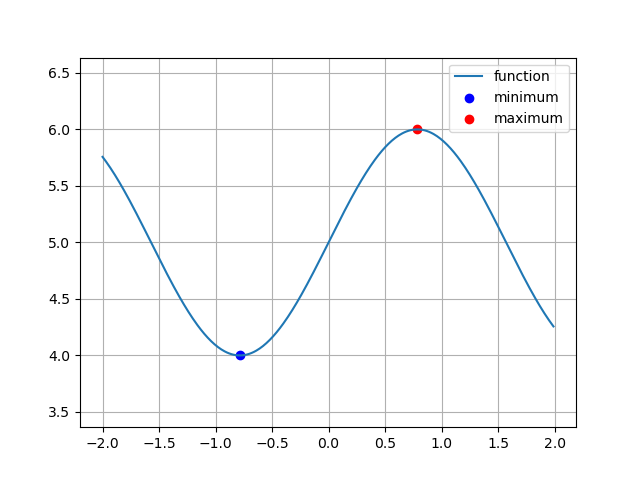
\includegraphics[width=\columnwidth]{figs/plot.png}
    \caption{local maximum and minimum}
    \label{fig:Plot1}
    \end{figure}
\end{document}}